% !TeX root = ../../../main.tex

We do not attempt to give a full review of the underlying theory
here as it is known since a long time and discussed extensive elsewhere
(see e.g.\ \cite{Peskin:1995ev,Ellis:1996mzs} and references therein).
We refer the interested reader to the specific references given in the following and to
the accompanying online documentation where instead we give a detailed
overview. All sections in the following have an equivalent section in
the online documentation. Also the respective code implementations of the
various ingredients contain relevant information and are also accessible
in the documentation via the API section.

The central equations that \eko{} is solving are the
Dokshitzer-Gribov-Lipatov-Altarelli-Parisi (\dglap) evolution
equations~\cite{Altarelli:1977zs,Gribov:1972ri,Dokshitzer:1977sg} given by
\begin{equation}
	\muF^2 \dv{\vb f}{\muF^2}{}(x,\muF^2) = \vb P (a_s(\muR^2),\muF^2) \otimes \vb f(\muF^2)
	\label{eq:eko/dglap}
\end{equation}
where $\vb f(x,\muF^2)$ is a vector of \pdfs over flavor space with $x$ the
momentum fraction and $\muF^2$ the factorization scale.
The main ingredients to \cref{eq:eko/dglap} are the Altarelli-Parisi splitting
functions $\vb P(a_s(\muR^2),x,\muF^2)$~\cite{Moch:2004pa,Vogt:2004mw}, which
are matrices over the flavor space.
Finally, $\otimes$ denotes the multiplicative (or Mellin) convolution.

The splitting functions $\vb P(a_s(\muR^2),x,\muF^2)$ expose a perturbative
expansion in the strong coupling $a_s(\mu_R^2)$:
\begin{align}
	\vb P(a_s(\muR^2),x,\muF^2) = a_s(\muR^2) \vb P^{(0)}(x,\muF^2)
	+ \qty[a_s(\muR^2)]^2 \vb P^{(1)}(x,\muF^2)
	+ \qty[a_s(\muR^2)]^3 \vb P^{(2)}(x,\muF^2)
	+ \ldots
\end{align}
which is currently known at \nnlo{}~\cite{Moch:2004pa,Vogt:2004mw,Blumlein:2021enk} and is under
investigation for \nnnlo{}~\cite{Moch:2021qrk}.
In a first step, the renormalization scale $\muR$ and the factorization scale
$\muF$ can be assumed to be equal $\muR = \muF$ and the renormalization scale
dependence can be restored later on. The variation of the ratio $\muR/\muF$ can
be considered as an estimated to missing higher order
uncertainties (\mhou{})~\cite{AbdulKhalek:2019ihb}.

In order to solve \cref{eq:eko/dglap} a series of steps has to be taken, and we
highlight these steps in the following sections.

\subsection{Mellin space}
\label{sec:theory:mellin}
The presence of the derivative on the left-hand-side and the convolution on the
right-hand-side turns \cref{eq:eko/dglap} into a set of coupled
integro-differential equations which are non-trivial to solve.

A possible strategy in solving \cref{eq:eko/dglap} is by tackling the problem
head-on and iteratively solve the integrals and the derivative by taking small
steps: we refer to this as \enquote{$x$-space solution}, as the solution uses
directly momentum space and this approach is adopted, e.g., by \apfel{}~\cite{Bertone:2013vaa},
\hoppet{}~\cite{Salam:2008qg}, and \qcdnum{}~\cite{Botje:2010ay}.
However, this approach becomes quite cumbersome when dealing with higher-order
corrections, as the solutions becomes more and more involved.

We follow a different strategy and apply the Mellin transformation $\Md$
\begin{equation}
    \tilde g(N) = \Md\qty[g(x)](N) = \int\limits_0^1\!\dd{x} x^{N-1} g(x)
\end{equation}
where, as well here as in the following, we denote objects in Mellin space by a
tilde.
This approach is also adopted by \pegasus{}~\cite{Vogt:2004ns} and \fk{}~\cite{Ball:2008by,Ball:2010de,DelDebbio:2007ee}.
The numerically challenging step is then shifted to the treatment of the Mellin
inverse $\Md^{-1}$, as we eventually seek for results in $x$-space (see
\cref{sec:theory:interpolation}).


\subsection{Interpolation}
\label{sec:theory:interpolation}
To bridge between the desired $x$-space input/output and the internal
Mellin representation, we do a Lagrange-Interpolation as sketched in
\cref{sec:theory:interpolation}
(and detailed in the \href{https://eko.readthedocs.io/en/latest/}{online documentation}).
We recommend a grid of at least 50 points with
linear scaling in the large-$x$ region ($x \gtrapprox 0.1$) and with logarithmic
scaling in the small-$x$ region and an interpolation of degree four.
Also the grids determined by \amcfast~\cite{Bertone:2014zva} perform
sufficiently well for specific processes.

\begin{figure}
    \begin{center}
    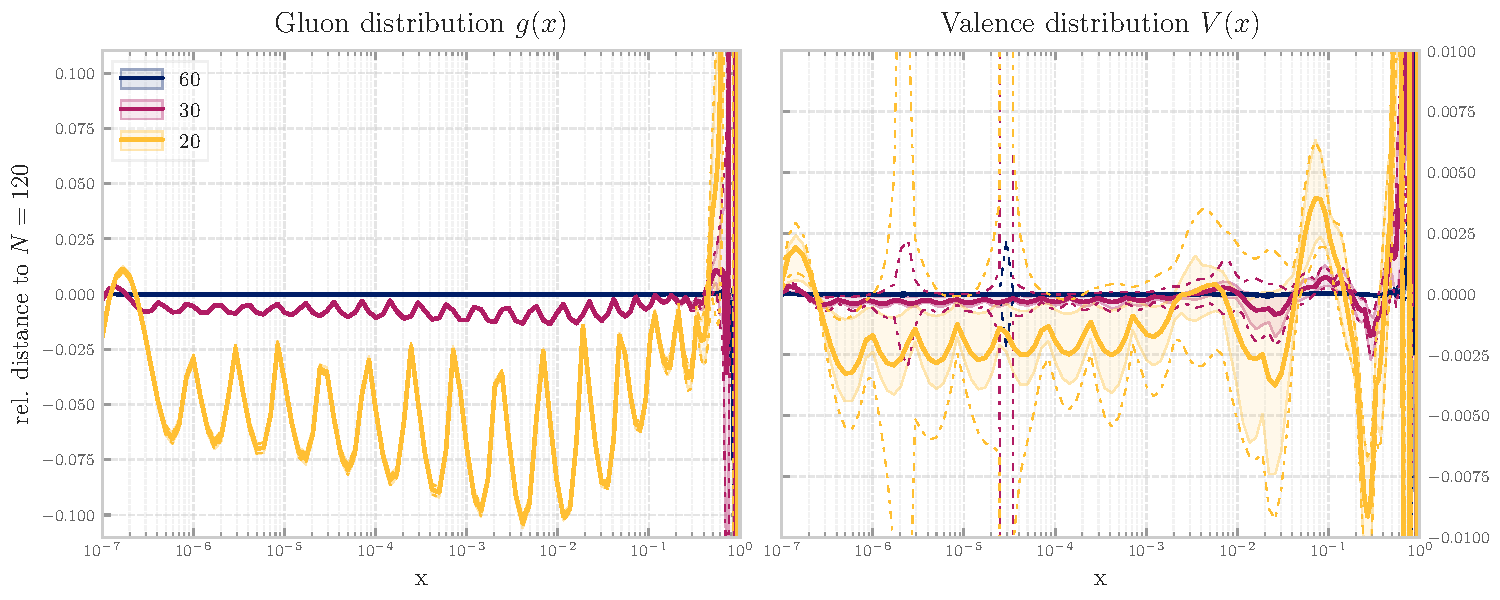
\includegraphics[width=\textwidth]{ch-eko/interpolation-int-ratio}
    \end{center}
    \caption{Relative differences between 
        the outcome of \nnlo{} \qcd{} evolution
        as implemented in \eko{} with 20, 30, and 60 points to 120
        interpolation points respectively.
        \label{fig:interpolation} }
\end{figure}

For a first qualitative study we show in \cref{fig:interpolation} a
comparison between an increasing number of interpolation points
distributed according to \cite[Eq. 2.12]{Carrazza_2020}.
The separate configurations are converging to the solution with the
largest number of points. Using 60 interpolation points is almost
indistinguishable from using 120 points (the reference configuration in the plot).
In the singlet sector (gluon) the convergence is
significantly slower due to the more involved solution strategies and,
specifically, the oscillating behavior is caused due to these difficulties.
The spikes for $x\to 1$ are not relevant since the \pdf{}s are intrinsically
small in this region ($\vb f\to 0$) and thus small numerical differences
are enhanced.

Also note that the results of \cref{sec:pheno:bench} (i.e.\ \cref{fig:LHAbench,fig:Apfelbench_pto,fig:Pegasusbench_pto}) confirm that
the interpolation error can be kept below the benchmark accuracy.


\subsection{Strong coupling}
\label{sec:theory:coupling}
The evolution of the strong coupling $a_s(\mu^2) = \alpha_s(\mu^2)/(4\pi)$
is given by its renormalization group equation (\rge):
\begin{equation}
    \beta(a_s) = \mu^2\dv{a_s(\mu^2)}{\mu^2}{} = - \sum\limits_{n=0} \beta_n \qty[a_s(\mu^2)]^{2+n}
\end{equation}
and is currently known at 5-loop ($\beta_4$)
accuracy~\cite{Herzog:2017ohr,Luthe:2016ima,Baikov:2016tgj,Chetyrkin:2017bjc,Luthe:2017ttg}.

This is crucial for \dglap{} solution, indeed, since the strong coupling $a_s$
is a monotonic function of the scale $\mu$ in the perturbative regime, we can
actually consider a transformation of
\cref{eq:eko/dglap}
\begin{equation}
    \dv{\vb{\tilde f}}{a_s}{}(N,a_s) = - \frac{\bm{\gamma}(N,a_s)}{\beta(a_s)} \vb {\tilde f}(N, a_s)
    \label{eq:eko/dglap2}
\end{equation}
with $\bm{\gamma} = - \vb{\tilde P}$ the anomalous dimension and $\beta(a_s)$
the \qcd{} beta function, where the multiplicative convolution is reduced to an
ordinary product.


\subsection{Flavor space}
\label{sec:theory:flavor}
Next, we address the separation in flavor space: formally we can define the
flavor space $\Fd$ as the linear span over all partons (which we consider to be
the canonical one):
\begin{equation}
    \Fd = \Fd_{fl} = \vspan\qty(g, u, \bar u, d, \bar d, s, \bar s, c, \bar c, b, \bar b, t, \bar t)
\end{equation}

The splitting functions $\vb P$ become block-diagonal in the \enquote{Evolution
Basis}, a suitable decomposition of the flavor space: the singlet sector $\vb
P_S$ remains the only coupled sector over $\qty{\Sigma, g}$, while the full
valence combination $P_{ns,v}$ decouples completely (i.e.\ it is only coupling
to $V$), and the non-singlet singlet-like sector $P_{ns,+}$ is diagonal over
$\qty{T_3,T_8,T_{15},T_{24},T_{35}}$, and the non-singlet valence-like sector
$P_{ns,-}$ is diagonal over $\qty{V_3,V_8,V_{15},V_{24},V_{35}}$.
The respective distributions are given by their usual definition.

This Evolution Basis is isomorphic to our canonical choice
\begin{equation}
    \Fd \sim \Fd_{ev} = \vspan(g, \Sigma, V, T_{3}, T_{8}, T_{15}, T_{24}, T_{35}, V_{3}, V_{8}, V_{15}, V_{24}, V_{35})
\end{equation}
but, it is not a normalized basis. When dealing with intrinsic evolution, i.e.\
the evolution of \pdf{}s below their respective mass scale, the Evolution Basis
is not sufficient. In fact, for example, $T_{15} = u^{+} + d^{+} +
s^{+} - 3c^{+}$ below the charm threshold $\mu_c^2$ contains both running and static
distributions which need to be further disentangled.

We are thus considering a set of \enquote{Intrinsic Evolution Bases} $\Fd_{iev,
n_f}$, where we retain the intrinsic flavor distributions as basis vectors.
The basis definition depends on the number of light flavors $n_f$ and, e.g.\
for $n_f=4$, we find
\begin{equation}
    \Fd \sim \Fd_{iev,4} = \vspan(g, \Sigma_{(4)}, V_{(4)}, T_{3}, T_{8}, T_{15}, V_{3}, V_{8}, V_{15}, b^+, b^-, t^+, t^-)
\end{equation}
with $\Sigma_{(4)} = \sum\limits_{j=1}^4 q_j^+$ and $V_{(4)} =
\sum\limits_{j=1}^4 q_j^-$.


\subsection{Solution Strategies}
\label{sec:theory:solutions}
The formal solution of \cref{eq:eko/dglap2} in terms of evolution kernel
operators $\vb {\tilde E}$ is given by
\begin{equation}
    \vb {\tilde E}(a_s \leftarrow a_s^0)  = \Pd \exp\qty[-\int\limits_{a_s^0}^{a_s} \frac{\bm{\gamma}(a_s')}{\beta(a_s')} \dd{a_s'} ]
    \label{eq:eko/eko}
\end{equation}
with $\Pd$ the path-ordering operator. If the anomalous dimension $\bm{\gamma}$ is
diagonal in flavor space, i.e.\ it is in the non-singlet sector, it is always
possible to find an analytical solution to \cref{eq:eko/eko}. 
In the singlet sector sector, however, this is only true at LO and to obtain a
solution beyond, we need to apply different approximations and solution
strategies, on which \eko{} offers currently eight implementations. For an
actual comparison of selected strategies, cf.\ \cref{sec:eko/pheno-sols}.


\subsection{Matching at Thresholds}
\label{sec:theory:matching}
\eko{} can perform calculation in a fixed flavor number scheme (\ffns{}) where
the number of active or light flavors $n_f$ is constant. This means that both
the beta function $\beta^{(n_f)}(a_s)$ and the anomalous dimension
$\bm{\gamma}^{(n_f)}(a_s)$ in \cref{eq:dglap2} are constant with respect to
$n_f$.
However, this approximation is likely to fail either in the high energy region
$\muF^2 \to \infty$ for a small number of active flavors, or to fail in the low
energy region $\muF^2 \to \Lambda_{\text{QCD}}^2$ for a large number of active
flavors.

This can be overcome by using a variable flavor number scheme (\vfns{}) that
changes the number of active flavors when the scale $\muF^2$ crosses a
threshold $\mu_h^2$.
This then requires a matching procedure when changing the number of active
flavors, and for the \pdf{}s we find
\begin{equation}
    \tilde{\mathbf{f}}^{(n_f+1)}(\mu_{F,1}^2)= \tilde{\mathbf{E}}^{(n_f+1)}(\mu_{F,1}^2\leftarrow \mu_{h}^2) {\mathbf{R}^{(n_f)}} \tilde{\mathbf{A}}^{(n_f)}(\mu_{h}^2) \tilde{\mathbf{E}}^{(n_f)}(\mu_{h}^2\leftarrow \mu_{F,0}^2) \tilde{\mathbf{f}}^{(n_f)}(\mu_{F,0}^2)
    \label{eq:matching}
\end{equation}
where the superscript refers to the number of active flavors and we split the matching into two
parts: the perturbative operator matrix elements (\ome{}) $\tilde{\mathbf{A}}^{(n_f)}(\mu_{h}^2)$,
currently implemented at \nnlo{}~\cite{Buza_1998}, and an algebraic rotation ${\mathbf{R}^{(n_f)}}$ acting
only in the flavor space $\Fd$.

For backward evolution this matching has to be applied in the reversed order.
The inversion of the basis rotation matrices $\mathbf{R}^{(n_f)}$ is simple,
whereas this is not true for the \ome{} $\mathbf{\tilde A}^{(n_f)}$ especially
in case of \nnlo{} or higher order evolution.
In \eko{} we have implemented two different strategies to perform the inverse
matching: the first one is a numerical inversion, where the OMEs are inverted
exactly in Mellin space, while in the second method, called \texttt{expanded},
the matching matrices are inverted through a perturbative expansion in $a_s$,
given by:
\begin{align}
    \qty(\mathbf{\tilde A}^{(n_f)})_{exp}^{-1}(\mu_{h}^2) &= \mathbf{I} - a_s(\mu_{h}^2) \mathbf{\tilde A}^{(n_f),(1)} + a_s^2(\mu_{h}^2) \qty[ \mathbf{\tilde A}^{(n_f),(2)} - \qty(\mathbf{\tilde A}^{(n_f),(1)})^2 ] + O(a_s^3)
    \label{eq:invmatchingexp}
\end{align}
with $\mathbf{I}$ the identity matrix in flavor space.


\subsection{Running Quark Masses}
\label{sec:theory:msbarmass}
In \cref{fig:eko/MSbarbench} we investigate the effect of adopting a running mass
scheme onto the respective \pdf{} sets. The left panel shows the $T_{15}(x)$
distribution obtained from the NNPDF4.0 perturbative charm
determination~\cite{NNPDF:2021njg} using the pole mass scheme and the \msbar{}
scheme, respectively.
The distributions have been evolved on $\muF^2=\SI[parse-numbers=false]{1\to
10^4}{\GeV^2}$.
The mass reference values are taken from
\cite{LHCHiggsCrossSectionWorkingGroup:2016ypw}, with the \msbar{}
boundary condition on the charm mass given as $m_c(\mu_m=\SI{3}{\GeV}) =
\SI{0.986}{\GeV}$, leading to $m_c(m_c) = \SI{1.265}{\GeV}$, while the charm
pole mass is $m^\text{pole}_{c}\approxeq\SI{1.51}{\GeV}$~\cite{NNPDF:2021njg}.
The major differences are visible in the low-x region where the \dglap{}
evolution is faster and the differences between the charm mass treatment are
enhanced: an higher value of the charm mass increases the singlet like
distribution $T_{15}(x)$.
For the sake of comparison, in the right panel, we plot the relative distance
to our result when comparing with the \apfel{}~\cite{Bertone:2013vaa}
implementation.
As expected the pole mass results are closer due to the same value of the charm
mass, while the \msbar{} results have a slightly bigger discrepancy which
remains in all the $x$-range around $1\permil$ accuracy.

\begin{figure}
    \centering
    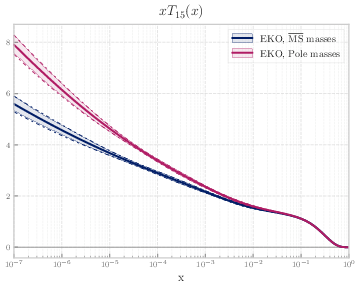
\includegraphics[width=0.47\linewidth]{ch-eko/msbar_T15.png}
    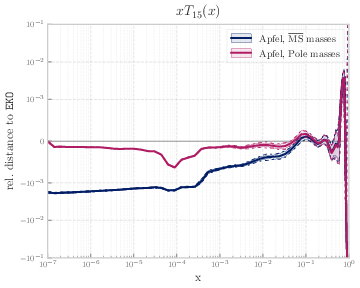
\includegraphics[width=0.47\linewidth]{ch-eko/msbar_bench_T15.png}
    \caption{(left) The NNPDF4.0 perturbative charm distribution
        $T_{15}(x)$~\cite{NNPDF:2021njg} with \msbar{} and pole masses \nnlo{}
        evolution when running on $\muF^2=\SI[parse-numbers=false]{1\to
        10^4}{\GeV^2}$.  (right) Relative difference to \eko{} for the same run
        with \apfel{}~\cite{Bertone:2013vaa}.}
     \label{fig:eko/MSbarbench}
\end{figure}

\begin{figure}
    \centering
    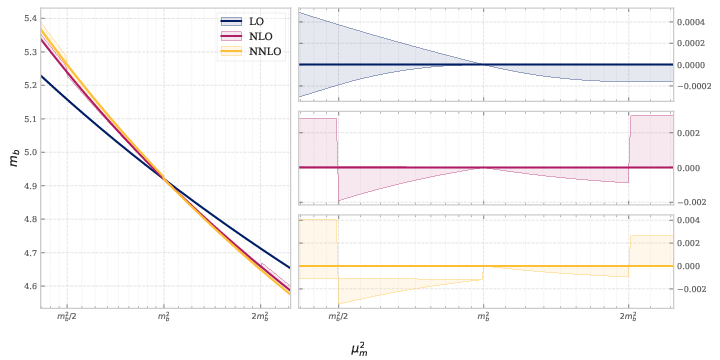
\includegraphics[width=\textwidth]{ch-eko/masses_running}
    \caption{Running of the bottom quark mass $m_b(\mu_m^2)$ for different threshold
        ratios, similar to \cref{fig:eko/asmatching}.
        The plot shows how the different choices of matching scales affect the
        running in the matching region (and slightly beyond) at \lo{}, \nlo{},
        and \nnlo{}.
        The border condition for the running has been chosen at $m_b(m_b) =
        \SI{4.92}{GeV}$, as it is clear from the plot, since it is the
        intersection point of all the curves shown.}
    \label{fig:eko/runningmasses}
\end{figure}


In \cref{fig:eko/runningmasses} we show the evolution of the \msbar{} bottom mass
$m_b(\mu_m^2)$ using different matching scales $\mu_b^2$ equal to $1/2,1$ and
$2$ times the mass $m_b^2$, for each perturbative order (\lo{}, \nlo{}, and
\nnlo{}).
The curve for $\mu_b^2 = m_b^2$ has been plotted as the central one (bold),
while the other two are used as the upper and lower borders of the shaded area
(according to their value, point by point).
The reference value $m_b(\mu_{b,0}^2)$, has been chosen equal for the
three curves, and it has been chosen at $m_b(m_b) = \SI{4.92}{GeV}$.
For this reason, above the central matching point $\mu_m^2 \ge m_b^2$ two curves coincide
($\mu_b^2 = m_b^2$ and $\mu_b^2 = m_b^2/2$) since they are both
running with the same number of flavors ($n_f=5$) and they have the same
border condition. The curve using $\mu_b^2 = 2m_b^2$, however, still runs with
a smaller number of flavors ($n_f=4$) and so does not match the former two.
In the lower region $\mu_m^2 < m_b^2$ this is not happening, because even
if the number of flavors is now the same,
the border condition is specified above matching for $\mu_b^2 = m_b^2$ (in
$n_f=5$).
So, starting from $m_b^2$ and going downward, the central choice $\mu_b^2 =
m_b^2$ is matched first and then evolved, while the higher scale choice
$\mu_b^2 = 2m_b^2$ immediately runs with four light flavors at $m_b^2$. Thus
the difference consists just in the matching.

